%!TEX root = ../main.tex
%\todo{Fix notation to distinguish between free disease and endemic}

To see the positivity invariance we have to make all coordinates zero except for
one. In \autoref{sys::DeterministicSystem}it is quickly observed that there is
invariance when $ S_p = L_p = I_p = 0 $, in the case when $ S_v = 0 $ or 
$ I_p = 0 $, the flow of dynamics is always positive. Therefore
\autoref{sys::DeterministicSystem} is positive invariant.

Let $\R^n_+$ the first octant of $\R ^ n$ and consider  
$$	{
	\Gamma:= 
		\left \{ 
			(S_p, L_p, I_p, S_v, I_v)^{\top} \in \R^5_+: \quad
			0\leq S_p + L_p + I_p \leq N_p, \quad
			S_v + I_v \leq \frac{\mu}{\gamma}
		\right \},
	}
$$
Here we compute the deterministic fixed points of system 
\eqref{sys::DeterministicSystem} and show that its unicity. Thus by definition of we solve 
%
\begin{equation}
	\begin{aligned}
		-\beta_p S_p \frac{I_v}{N_v} + r(N_p-S_p) &= 0\\
		\beta_p S_p \frac{I_v}{N_v} - b L_p - r L_p &= 0\\
		b L_p - r I_p &= 0\\
		-\beta_v S_v \frac{I_p}{N_p} -\gamma S_v +(1-\theta) \mu &= 0\\
		\beta_v S_v \frac{I_p}{N_p} -\gamma I_v + \theta \mu &= 0.
	\end{aligned}
\end{equation}
to determine our fixed points.
%
There is two fixed points\textemdash free disease equilibrium and the 
endemic equilibrium. We characterize the fist the relation
$ L^*_p=I_p^*=I_v^*=0$, which implies that
%
\begin{equation*}
	r(N_p-S^*_p) = 0,
\end{equation*}
%
and therefore, we obtain $S_p^*=N_p$.F or the vector population we have by 
\autoref{thm::conservationlaw} that $S_v^*+I_v^* \rightarrow \frac{\mu}{\gamma}$ as 
$\rightarrow \infty$, then $S_v^* \rightarrow \frac{\mu}{\gamma}$ when we have 
$I^*_v=0$.
%
The free disease equilibrium point is $(N_p,0,0,\frac{\mu}{\gamma},0)^{\top}$. 
For the case of endemic equilibrium point, we need suppose that $L_p^{**},I_p^{**},I_
v^{**}\neq0$ and solve each right hand side of system \autoref{sys::DeterministicSystem} in terms
of other variable.
%
From $\dot{S_p}$, we can obtain
%
\begin{equation*}
	S^{**}_p= \frac{rN_{{p}}N_{{v}}}{rN_{{v}}+I^{**}_v\beta_{{p}}},
\end{equation*}
%
 and similar for the other equations we obtain
\begin{equation*}
	\begin{aligned}
		L^{**}_p &= \frac{\beta_{{p}}S_p^{**} I_v^{**}}{N_{{v}} \left( b+r \right)},
		\\
		I^{**}_p &=\frac{b L^{**}_p}{r},
		\\
		S^{**}_v &=
			\frac{
				\left( 
					1-\theta 
				\right) 
				\mu\, N_{p}
			}{
				\gamma\, N_{p} + I^{**}_ p
				\beta_{v}
			},
	\end{aligned}
\end{equation*}
%
Expresing the above coordinate in terms of $I^{**}_v$, we obtain
%
%\improvement{rewrite as align}
%
\begin{equation*}
	\begin{aligned}
	S^{**}_p &= 
		\frac{
			r N_p N_v
		}{
			r N_v + 
			I^{**}_v 
			\beta_p
		},
	\\
	L^{**}_p &= 
		\frac{
			\beta_p rN_p I^{**}_v
		}{
			\left( 
				b + r 
			\right)
			(
				r N_v + I_v^{**} 
				\beta_p
			)
		},
%
%
	\\
	I^{**}_p &=
		\frac{
			b \beta_p N_p I_v^{**}
		}{
			 \left(
			 	 b + r 
			 \right)
			 ( r N_v + 
			 	I_v^{**} \beta_p
			 )
		},
	\\
	S^{**}_v &=
		\frac{
			 \left( 
			 	1 - \theta 
			 \right)
			 \mu(b + r)
			 (rN_v + \beta_p I_v^{**})
		}{
			\gamma(b + r)
			(r N_v + \beta_p I^{**}_v) + 
			b \beta_p \beta_v I_v^{**}
		},
	\end{aligned}
\end{equation*}
%
%
We only need substituting the above expression into the differential equation 
of $I_v$ and solve the following quadratic equation
%
	\begin{multline}
		-N_p [ 
			b \gamma^2 r I^{**}_v N_v +
			b \gamma^2 (I^{**}_v)^2 \beta_p -
			b \gamma \mu r \theta N_v - 
			b \gamma \mu \theta I^{**}_v \beta_p + 
			\\
			b \gamma (I^{**}_v)^2 \beta_p \beta_v + 
			b \mu \theta I^{**}_v \beta_p ^ 2
			-
			b \mu \theta I^{**}_v \beta_p \beta_v +
			\gamma^2 r^2 I^{**}_v N_v +
			\\
			\gamma^2 r (I ^{**}_v) ^ 2 \beta_p - 
			\gamma\mu r^2 \theta N_v - 
			\gamma\mu r \theta I^{**}_v +
			\beta_p - b\mu I^{**}_v \beta_p^2
		] = 0 \ .
	\end{multline}
% 
In sake of clearness we define 
\begin{align*}
	a_1 &:= 
		b \gamma^2 \beta_p + 
		b \gamma \beta_p \beta_v + 
		\gamma^2 r \beta_p
		,\\
	a_2 &:=-b \gamma \mu \theta \beta_p + 
		b \mu \theta \beta_p ^ 2 - 
		b \mu \theta \beta_p \beta_v + 
		\gamma^2 r^2 N_v - 
		\gamma \mu r 
		\theta \beta_p - 
		b \mu \beta_p^ 2 + 
		\gamma ^ 2 r N_v,
	\\
	a_3 &:=-b\gamma\mu r\theta N_v-\gamma\mu r^2\theta N_v, 
\end{align*}
%
and rewrite the above equation in this new notation as

\begin{equation}\label{eqn::QuadraticInfectedFP}
    \begin{aligned}
    	&\underbrace{
    		(
    		b \gamma^2 \beta_p + 
    		b \gamma \beta_p \beta_v + 
    		\gamma^2 r \beta_p
    		)
    	    }_{:=a_1} I_v^{**2}\\
    	&+ 
    	\underbrace{
    	(-b \gamma \mu \theta \beta_p + 
    		b \mu \theta \beta_p ^ 2 - 
    		b \mu \theta \beta_p \beta_v + 
    		\gamma^2 r^2 N_v - 
    		\gamma \mu r 
    		\theta \beta_p - 
    		b \mu \beta_p^ 2 + 
    		\gamma ^ 2 r N_v
    		)
    		}_{:=a_2} I^{**}_v \\
    		&- 
    	\underbrace{
    	(b\gamma\mu r\theta N_v+\gamma\mu r^2\theta N_v
    	)}_{:=a_3}=0 \ .
\end{aligned}
\end{equation}

%\todo{Fill according to each term}
We need a positive solution, then according to discriminant, we obtain
\begin{equation*}
	\begin{aligned}
		\Delta &= 
		a_2  ^ 2 -  4a_1 a_3
		\\
		&=
			(
				- b \gamma \mu \theta \beta_p +
				b \mu \theta \beta_p^2 -
				b \mu \theta \beta_p \beta_v + 
				\gamma ^ 2 r ^ 2 N_v - 
				\gamma \mu r \theta \beta_p - 
				b \mu \beta_p ^ 2 + 
				\gamma ^ 2 r N_v 
			) ^ 2
		\\
		& +  
		%
		4( 
			b \gamma ^ 2 \beta_p + 
			b \gamma \beta_p
			\beta_v + 
			\gamma^2 r \beta_p
		)
		%
		(
			b \gamma \mu r 
			\theta N_v + 
			\gamma \mu r ^ 2 \theta N_v
		),			
	\end{aligned}	
\end{equation*}
which ever is positive, then we have two different real solution, 
since we require the positive, we deduce that
\begin{equation*}
	I^{**}_{v} = 
		\frac{
			-a_2 + 
			\sqrt{a_2^2 - 4a_1 a_3}}%
		{2a_1}.
\end{equation*}
In \cite{VandenDriessche2017} we can find in detail the calculation of the $ \mathcal{R}^d_0$
which we define as the spectral radius of the next generation matrix, for the
system\autoref{sys::DeterministicSystem} we have the next matrix generation is

\begin{equation}\label{Mtx::NextGenerationMatrix}
    K:=
        \begin{bmatrix}
        0 & 0 &\frac{\beta_p S^*_p}{N_v \gamma} \\
        0 & 0 & 0 \\
        \frac{\beta_v S^*_v b}{(N_p (b+r_1) r_2} & \frac{\beta_v S^*_v}{(N_p r_2} & 0\\
        \end{bmatrix},
\end{equation}
%
matrix $K$  has $(i, j)$ entry equal to the expected number of secondary infections in compartment $i$
produced by an infected individual introduced in compartment $j$. Calculating the basic reproductive
number for the system \autoref{sys::DeterministicSystem} we have

\begin{equation}\label{eqn::DeterministicBRN}
    \mathcal{R}^d_0:=\sqrt{\frac{\beta_p \beta_v b}{(b + r_1 ) r_2 \gamma}}.
\end{equation}

In \cite{VandenDriessche2017}, they prove that under the condition of $\mathcal{R}^d_0$
we can established the stability of the free disease fixed point, then we can obtain the following result

\begin{theorem}\label{Thm::StabilityFreePointBasicReproNumberDeter}
If $\mathcal{R}^d_0 < 1$, the free disease fixed point $FE$ of model \autoref{sys::DeterministicSystem}
is locally asymptotically stable, and is unstable if $\mathcal{R}^d_0>1$.
\end{theorem}

In the case when $\mathcal{R}^d_0>1$ we have the instability of free disease fixed point,
but we obtain the stability of the endemic fixed point, and we can established the following result
\info{include references to Theroems. Thm or pages}

\begin{theorem}{\cite[Thm. ][]{}}
\label{Thm::StabilityEndemicPointBasicReproNumberDeter}
If $\mathcal{R}^d_0>1$, the endemic equilibrium  of system \autoref{sys::DeterministicSystem}
is locally asymptotically stable.
\end{theorem}
\info{Write a paragraph to describe Fig.1 according to data and simulation}

\begin{figure}[h]
	\centering	
	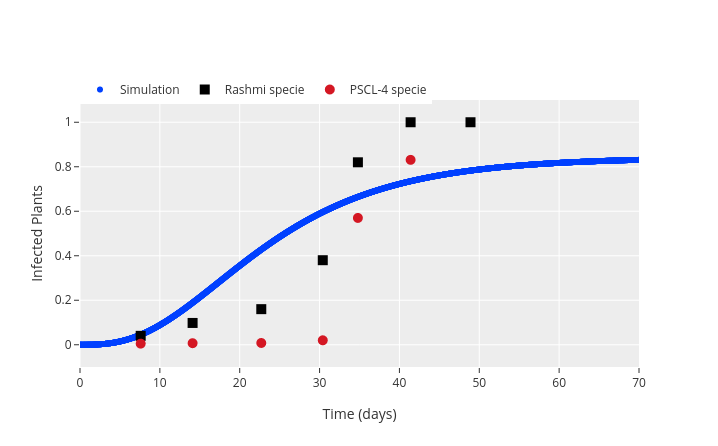
\includegraphics[scale=0.385, keepaspectratio]{%
	Figures/Tomato_with_data.png}
	\caption{Infected Plant population with two types of tomato species. The curve represent
	a susceptible variety of tomato the parameters are taking of deterministic case of table
	\autoref{tbl:value}, $\mathcal{R}^d_0>1$.
		\href{https://plotly.com/~AdrianSalcedo/24/}{
		https://plotly.com/~AdrianSalcedo/24/}}
	\label{fig:Deterministic_Infected_with_data}
\end{figure}